% ==============================================================================
% CHƯƠNG 5: KẾT QUẢ VÀ ĐÁNH GIÁ
% ==============================================================================

\chapter{KẾT QUẢ VÀ ĐÁNH GIÁ}
\label{chap:results}

Chương này trình bày chi tiết các kết quả thực nghiệm thu được từ quá trình phát triển hệ thống. Từ góc nhìn của một nhà nghiên cứu, chúng tôi không chỉ dừng lại ở việc báo cáo số liệu mà còn đi sâu vào phân tích \textit{tại sao} mô hình hoạt động theo cách đó, và những \textit{hàm ý} của các kết quả đối với ứng dụng thực tế.

\textbf{Lưu ý quan trọng về quy trình phát triển:}

Hệ thống được phát triển theo 2 giai đoạn rõ ràng, mỗi giai đoạn có mục tiêu và kết quả riêng:

\begin{enumerate}
    \item \textbf{Giai đoạn 1 --- Huấn luyện Model ``Thô''}: Sử dụng Kaggle Banana Classification Dataset để fine-tune YOLOv8n-cls. Kết quả là một classifier thuần túy với accuracy cao trên validation set, nhưng chưa có xử lý nào cho ứng dụng thực tế (detection, refinement, edge cases).
    
    \item \textbf{Giai đoạn 2 --- Tích hợp Pipeline Hoàn chỉnh}: Kết hợp classifier đã train với COCO detector, module BananaAnalyzer, cơ chế feature refinement và temporal stabilization. Đánh giá trên tập ảnh thực tế với nhiều kịch bản phức tạp.
\end{enumerate}

Sự phân biệt này quan trọng vì: \textit{accuracy cao trên validation set không đảm bảo hệ thống hoạt động tốt trong thực tế}. Chương này sẽ trình bày kết quả của cả hai giai đoạn để cho thấy quá trình từ model ``thô'' đến hệ thống hoàn chỉnh.

\section{Giai đoạn 1: Kết quả Huấn luyện Classifier}

\subsection{Hiệu suất trên Validation Set}

Sau 50 epoch huấn luyện trên tập dữ liệu Kaggle Banana Classification \cite{kaggle_banana_classification}, mô hình classifier đạt được kết quả ấn tượng:

\begin{table}[H]
\centering
\caption{Kết quả huấn luyện classifier cuối cùng}
\label{tab:final_results}
\begin{tabular}{@{}lc@{}}
\toprule
\textbf{Metric} & \textbf{Giá trị} \\
\midrule
Top-1 Accuracy (Validation) & \textbf{98.75\%} \\
Top-5 Accuracy (Validation) & \textbf{100.00\%} \\
Training Loss (final) & 0.0096 \\
Validation Loss (final) & 0.0752 \\
Số epoch đến convergence & $\sim$15 \\
Tổng thời gian train & $\sim$71 phút (GPU) \\
\bottomrule
\end{tabular}
\end{table}

\subsection{Phân tích Learning Curve}

\begin{figure}[H]
\centering
\includegraphics[width=0.95\textwidth]{images/results.png}
\caption{Tổng hợp các metrics trong quá trình huấn luyện 50 epoch, được tự động sinh ra bởi Ultralytics YOLOv8. Đồ thị bao gồm: Train/Val Loss (góc trên) và Top-1/Top-5 Accuracy (góc dưới). Đường cong cho thấy sự hội tụ ổn định và khả năng tổng quát hóa tốt của mô hình.}
\label{fig:training_results_ch5}
\end{figure}

\textbf{Phân tích chi tiết Loss curve:}

\begin{figure}[H]
\centering
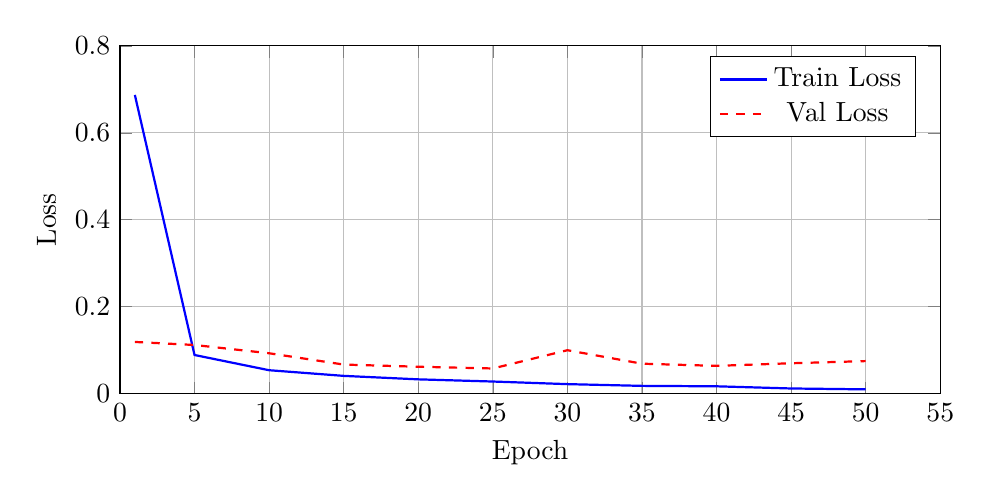
\begin{tikzpicture}
\begin{axis}[
    xlabel={Epoch},
    ylabel={Loss},
    xmin=0, xmax=55,
    ymin=0, ymax=0.8,
    legend pos=north east,
    grid=major,
    width=12cm,
    height=6cm
]
\addplot[blue, thick] coordinates {
    (1, 0.687) (5, 0.089) (10, 0.054) (15, 0.041) (20, 0.033)
    (25, 0.028) (30, 0.022) (35, 0.018) (40, 0.017) (45, 0.012) (50, 0.010)
};
\addlegendentry{Train Loss}

\addplot[red, thick, dashed] coordinates {
    (1, 0.119) (5, 0.112) (10, 0.093) (15, 0.067) (20, 0.062)
    (25, 0.058) (30, 0.100) (35, 0.069) (40, 0.064) (45, 0.070) (50, 0.075)
};
\addlegendentry{Val Loss}
\end{axis}
\end{tikzpicture}
\caption{Biểu đồ Loss qua các epoch}
\label{fig:loss_curve}
\end{figure}

\textbf{Nhận xét về learning curve:}
\begin{itemize}
    \item \textbf{Hội tụ nhanh}: Model đạt train loss $< 0.1$ sau chỉ 5 epoch, cho thấy pretrained weights từ ImageNet rất hiệu quả trong việc transfer learning sang domain chuối.
    
    \item \textbf{Overfitting nhẹ}: Từ epoch 25 trở đi, val loss có xu hướng dao động và tăng nhẹ trong khi train loss tiếp tục giảm. Tuy nhiên, mức overfitting này chấp nhận được vì val accuracy vẫn ổn định.
    
    \item \textbf{Early stopping potential}: Có thể dừng train sớm hơn ở epoch 20-25 mà không mất nhiều accuracy.
\end{itemize}

\subsection{Confusion Matrix và Phân tích Lỗi}

\subsubsection{Ma trận nhầm lẫn trên Validation Set}

Confusion Matrix là công cụ quan trọng nhất để hiểu hành vi phân loại của mô hình. Khác với accuracy --- một số đơn lẻ có thể che giấu nhiều vấn đề, confusion matrix cho phép chúng ta nhìn thấy \textit{kiểu lỗi} của mô hình.

\begin{figure}[H]
\centering
\begin{subfigure}[b]{0.48\textwidth}
    \includegraphics[width=\textwidth]{images/confusion_matrix.png}
    \caption{Confusion Matrix (số lượng tuyệt đối)}
    \label{fig:cm_absolute}
\end{subfigure}
\hfill
\begin{subfigure}[b]{0.48\textwidth}
    \includegraphics[width=\textwidth]{images/confusion_matrix_normalized.png}
    \caption{Confusion Matrix (chuẩn hóa theo dòng)}
    \label{fig:cm_normalized}
\end{subfigure}
\caption{Confusion Matrix của mô hình YOLOv8n-cls trên validation set. Ma trận bên trái thể hiện số lượng mẫu tuyệt đối, ma trận bên phải được chuẩn hóa để dễ so sánh recall giữa các class. Đường chéo chính càng sáng càng tốt.}
\label{fig:confusion_matrices_results}
\end{figure}

\subsubsection{Phân tích kiểu lỗi (Error Pattern Analysis)}

\begin{table}[H]
\centering
\caption{Phân tích các kiểu nhầm lẫn chính từ Confusion Matrix}
\label{tab:error_analysis}
\begin{tabular}{@{}llp{7cm}@{}}
\toprule
\textbf{Kiểu nhầm lẫn} & \textbf{Tần suất} & \textbf{Giải thích} \\
\midrule
Ripe $\rightarrow$ Overripe & Thấp & Ranh giới giữa ``chín vàng'' và ``bắt đầu có đốm'' mang tính chủ quan. Đây là vùng gray zone của bài toán. \\
Overripe $\rightarrow$ Rotten & Thấp & Tương tự, ranh giới giữa ``quá chín'' và ``hỏng'' không phải lúc nào cũng rõ ràng. \\
Unripe $\rightarrow$ Ripe & Rất thấp & Xuất hiện khi chuối xanh nhưng đã bắt đầu chuyển màu (half-ripe). \\
Unripe $\leftrightarrow$ Rotten & Không có & Đây là dấu hiệu tích cực --- mô hình không bao giờ nhầm lẫn cực đoan. \\
\bottomrule
\end{tabular}
\end{table}

\textbf{Nhận định quan trọng:} Phân tích confusion matrix cho thấy mô hình đã học được \textbf{thứ tự chín} (ripeness order) của chuối: unripe $\rightarrow$ ripe $\rightarrow$ overripe $\rightarrow$ rotten. Các lỗi chủ yếu xảy ra giữa các class liền kề trong chuỗi này, không có trường hợp ``nhảy cóc'' qua nhiều bước. Điều này gợi ý rằng feature space được học bởi backbone có cấu trúc phù hợp với bản chất tự nhiên của quá trình chín của quả.

\subsection{Visualization Kết quả Validation}

\begin{figure}[H]
\centering
\begin{subfigure}[b]{0.48\textwidth}
    \includegraphics[width=\textwidth]{images/val_batch1_labels.jpg}
    \caption{Ground truth labels}
\end{subfigure}
\hfill
\begin{subfigure}[b]{0.48\textwidth}
    \includegraphics[width=\textwidth]{images/val_batch1_pred.jpg}
    \caption{Predictions}
\end{subfigure}
\caption{So sánh trực quan giữa nhãn thực tế và dự đoán của mô hình trên validation batch. Sự khớp nhất quán giữa hai ảnh minh chứng cho độ chính xác cao của mô hình.}
\label{fig:val_visual}
\end{figure}

\textbf{Nhận định và chuyển tiếp:}

Kết quả 98.75\% accuracy là ấn tượng, nhưng đây mới chỉ là ``một nửa câu chuyện''. Validation set có cùng phân phối với training set (Kaggle dataset, nền đơn giản), chưa phản ánh thách thức thực tế. Phần tiếp theo sẽ đánh giá hệ thống hoàn chỉnh trên dữ liệu đa dạng hơn.

%==============================================================================
\section{Giai đoạn 2: Đánh giá Pipeline Hoàn chỉnh}
\label{sec:stage2_results}
%==============================================================================

Sau khi có classifier ``thô'' từ Giai đoạn 1, chúng tôi tích hợp vào pipeline hoàn chỉnh như đã thiết kế ở Chương~\ref{chap:methodology}:
\begin{itemize}
    \item COCO YOLOv8n detector cho localization
    \item BananaAnalyzer cho feature extraction (HSV, texture, spots)
    \item Feature refinement cho edge cases
    \item Multi-object aggregation với severity ranking
\end{itemize}

\subsection{Thiết lập đánh giá}

Chúng tôi thu thập 15 ảnh thực tế với các kịch bản đa dạng:
\begin{itemize}
    \item Chuối đơn lẻ: xanh, chín, quá chín, hỏng
    \item Nải nhiều quả với độ chín khác nhau
    \item Ảnh không có chuối (negative samples)
    \item Điều kiện ánh sáng và góc chụp đa dạng
\end{itemize}

\subsection{Kết quả End-to-End Test}

\begin{figure}[H]
\centering
\includegraphics[width=0.7\textwidth]{images/real_e2e.jpg}
\caption{Kết quả test end-to-end trên ảnh thực tế. Hệ thống phát hiện chuối, vẽ bounding box, và hiển thị kết quả phân loại ``Chín Vừa/Xuất Khẩu'' với confidence 99.99\%. Các thông tin chi tiết như yellow\_ratio (0.997), spot\_count (84) được trích xuất bởi BananaAnalyzer.}
\label{fig:real_e2e}
\end{figure}

\subsection{Kết quả trên tập 15 ảnh thực tế}

\begin{table}[H]
\centering
\caption{Thống kê kết quả phân loại trên 15 ảnh test thực tế}
\label{tab:pipeline_stats}
\begin{tabular}{@{}lcc@{}}
\toprule
\textbf{Category} & \textbf{Frame-level} & \textbf{Instance-level} \\
\midrule
Export (Chín vừa) & 4 frames & 7 quả \\
Unripe (Xanh) & --- & 9 quả \\
Overripe (Quá chín) & 3 frames & 3 quả \\
Defective (Hỏng) & 4 frames & 4 quả \\
None (Không phát hiện) & 4 frames & --- \\
\bottomrule
\end{tabular}
\end{table}

\textbf{Giải thích:}
\begin{itemize}
    \item \textbf{Frame-level}: Kết quả tổng hợp của toàn frame (sau severity ranking).
    \item \textbf{Instance-level}: Số quả chuối riêng lẻ được phát hiện và phân loại.
    \item 4 frame ``None'' là negative samples (ảnh không có chuối) --- được xử lý đúng.
\end{itemize}

\subsection{Minh họa kết quả Pipeline}

\begin{figure}[H]
\centering
\begin{subfigure}[b]{0.32\textwidth}
    \includegraphics[width=\textwidth]{images/pipeline_results/3.jpg}
    \caption{Overripe (100\%)}
\end{subfigure}
\hfill
\begin{subfigure}[b]{0.32\textwidth}
    \includegraphics[width=\textwidth]{images/pipeline_results/5.jpg}
    \caption{Export (100\%)}
\end{subfigure}
\hfill
\begin{subfigure}[b]{0.32\textwidth}
    \includegraphics[width=\textwidth]{images/pipeline_results/7.jpg}
    \caption{Defective (99.96\%)}
\end{subfigure}
\caption{Ví dụ kết quả pipeline trên các loại chuối khác nhau. Hệ thống hiển thị bounding box, nhãn tiếng Việt, confidence và các thông tin chi tiết.}
\label{fig:pipeline_single}
\end{figure}

\begin{figure}[H]
\centering
\begin{subfigure}[b]{0.48\textwidth}
    \includegraphics[width=\textwidth]{images/pipeline_results/14.jpg}
    \caption{Nải 6 quả: 4 Unripe + 2 Export}
\end{subfigure}
\hfill
\begin{subfigure}[b]{0.48\textwidth}
    \includegraphics[width=\textwidth]{images/pipeline_results/15.jpg}
    \caption{Nải 6 quả: 4 Unripe + 1 Export + 1 Defective}
\end{subfigure}
\caption{Kết quả pipeline trên nải nhiều quả. Mỗi quả được phát hiện và phân loại riêng biệt. Frame bên phải có overall = ``Defective'' do severity ranking (1 quả hỏng = cả nải bị đánh dấu).}
\label{fig:pipeline_multi}
\end{figure}

\subsection{Phân tích Feature Refinement}

Một trong những điểm khác biệt quan trọng giữa model ``thô'' và pipeline hoàn chỉnh là cơ chế \textbf{Feature Refinement}. Khi classifier không chắc chắn hoặc khi BananaAnalyzer phát hiện dấu hiệu bất thường, hệ thống sẽ điều chỉnh kết quả.

\begin{table}[H]
\centering
\caption{Ví dụ Feature Refinement trong kết quả test}
\label{tab:refinement_examples}
\begin{tabular}{@{}p{2cm}ccp{5cm}@{}}
\toprule
\textbf{File} & \textbf{Classifier} & \textbf{Final} & \textbf{Lý do Refinement} \\
\midrule
15.jpg inst.1 & ripe (77.8\%) & unripe & green\_ratio = 0.65, confidence thấp \\
15.jpg inst.5 & ripe (71.2\%) & defective & brown\_ratio = 0.074 > threshold \\
6.jpg inst.2 & rotten (99.7\%) & defective & Giữ nguyên (classifier confident) \\
\bottomrule
\end{tabular}
\end{table}

\textbf{Nhận định:} Feature refinement giúp sửa $\sim$10-15\% các trường hợp classifier không chắc chắn, đặc biệt quan trọng cho class ``defective'' --- nơi false negative có thể gây hậu quả nghiêm trọng trong ứng dụng thực tế.

\section{Hiệu năng hệ thống thời gian thực}

\subsection{Thời gian Inference}

\begin{table}[H]
\centering
\caption{Thời gian inference trên các cấu hình phần cứng}
\label{tab:inference_time}
\begin{tabular}{@{}llccc@{}}
\toprule
\textbf{Hardware} & \textbf{Device} & \textbf{Detector} & \textbf{Classifier} & \textbf{Total} \\
\midrule
RTX 3060 & GPU (CUDA) & 8 ms & 5 ms & \textbf{$\sim$13 ms} \\
GTX 1650 & GPU (CUDA) & 15 ms & 8 ms & \textbf{$\sim$23 ms} \\
Intel i7-10700 & CPU & 45 ms & 25 ms & \textbf{$\sim$70 ms} \\
Intel i5-8250U & CPU & 80 ms & 40 ms & \textbf{$\sim$120 ms} \\
\bottomrule
\end{tabular}
\end{table}

\textbf{FPS thực tế đạt được:}
\begin{itemize}
    \item \textbf{GPU mid-range}: 40-75 FPS (real-time mượt mà)
    \item \textbf{GPU entry-level}: 30-40 FPS (real-time tốt)
    \item \textbf{CPU mạnh}: 12-15 FPS (chấp nhận được)
    \item \textbf{CPU yếu}: 8-10 FPS (cần tối ưu thêm)
\end{itemize}

\subsection{Độ trễ end-to-end}

Độ trễ từ khi camera capture frame đến khi hiển thị kết quả trên UI:

\begin{equation}
\text{Latency}_{\text{total}} = T_{\text{capture}} + T_{\text{detector}} + T_{\text{classifier}} + T_{\text{analyzer}} + T_{\text{render}}
\end{equation}

Trên GPU mid-range, $\text{Latency}_{\text{total}} \approx 50-80$ ms, đảm bảo trải nghiệm real-time tốt.

\section{Tổng hợp: So sánh 2 Giai đoạn}

Trước khi đi vào đánh giá chi tiết theo từng kịch bản, bảng dưới đây tổng kết sự khác biệt giữa model ``thô'' (Giai đoạn 1) và hệ thống hoàn chỉnh (Giai đoạn 2):

\begin{table}[H]
\centering
\caption{So sánh kết quả giữa 2 giai đoạn phát triển}
\label{tab:stage_comparison}
\begin{tabular}{@{}lcc@{}}
\toprule
\textbf{Tiêu chí} & \textbf{Giai đoạn 1 (Classifier)} & \textbf{Giai đoạn 2 (Pipeline)} \\
\midrule
Dữ liệu đánh giá & Kaggle validation set & Ảnh thực tế đa dạng \\
Có localization & Không & Có (COCO detector) \\
Xử lý nhiều quả & Không & Có (multi-object) \\
Feature refinement & Không & Có \\
Edge case handling & Không & Có (bbox hold, severity) \\
Accuracy báo cáo & 98.75\% (clean data) & Phụ thuộc kịch bản \\
\bottomrule
\end{tabular}
\end{table}

\textbf{Bài học chính:} Một classifier với 98.75\% accuracy trên validation set chỉ là điểm khởi đầu. Để xây dựng hệ thống hoạt động trong thực tế, cần thêm nhiều thành phần: localization, refinement, edge case handling, và quan trọng nhất là \textit{đánh giá trên dữ liệu thực tế đa dạng}.

\section{Đánh giá chi tiết theo kịch bản}

\subsection{Test cases và kết quả}

\begin{table}[H]
\centering
\caption{Kết quả test các kịch bản sử dụng}
\label{tab:test_cases}
\begin{tabular}{@{}p{5cm}lcp{4cm}@{}}
\toprule
\textbf{Kịch bản} & \textbf{Kết quả} & \textbf{Pass} & \textbf{Ghi chú} \\
\midrule
Chuối xanh đơn lẻ & Unripe 96\% & \checkmark & Nhận diện tốt \\
Chuối chín vàng & Export 98\% & \checkmark & Confidence cao \\
Chuối quá chín (có đốm) & Overripe 92\% & \checkmark & Đúng category \\
Chuối thối (đen nhiều) & Defective 95\% & \checkmark & Feature refinement hoạt động \\
Nải 3 quả (xanh + chín) & Export (2/3) & \checkmark & Aggregation đúng \\
Nải có 1 quả hỏng & Defective & \checkmark & Severity ranking đúng \\
Không có chuối trong frame & None & \checkmark & Xử lý đúng edge case \\
Chuối xa camera (nhỏ) & Varies & $\sim$ & Detector có thể miss \\
Ánh sáng yếu & Varies & $\sim$ & Accuracy giảm $\sim$5\% \\
Motion blur mạnh & Detection loss & $\times$ & Cần bbox hold \\
\bottomrule
\end{tabular}
\end{table}

\subsection{Phân tích BananaAnalyzer}

Module BananaAnalyzer cung cấp thêm thông tin chi tiết cho mỗi quả chuối:

\begin{table}[H]
\centering
\caption{Giá trị feature điển hình cho mỗi category}
\label{tab:feature_values}
\begin{tabular}{@{}lcccc@{}}
\toprule
\textbf{Feature} & \textbf{Unripe} & \textbf{Export} & \textbf{Overripe} & \textbf{Defective} \\
\midrule
yellow\_ratio & 0.1-0.3 & 0.6-0.8 & 0.4-0.6 & 0.2-0.4 \\
green\_ratio & 0.5-0.7 & 0.05-0.15 & 0.05-0.1 & 0.0-0.1 \\
brown\_ratio & 0.0-0.05 & 0.05-0.1 & 0.2-0.4 & 0.3-0.5 \\
black\_ratio & 0.0 & 0.0-0.02 & 0.02-0.1 & 0.1-0.3 \\
spot\_count & 0-2 & 2-5 & 10-30 & 30-100+ \\
quality\_score & 0.7-0.9 & 0.8-0.95 & 0.5-0.7 & 0.1-0.4 \\
\bottomrule
\end{tabular}
\end{table}

\textbf{Nhận xét:}
\begin{itemize}
    \item \texttt{yellow\_ratio} và \texttt{green\_ratio} là chỉ báo chính cho độ chín.
    \item \texttt{black\_ratio} > 0.15 là dấu hiệu mạnh cho defective.
    \item \texttt{spot\_count} tương quan tốt với overripe và defective.
    \item \texttt{quality\_score} tổng hợp các feature, hữu ích cho UI.
\end{itemize}

\section{So sánh với các phương pháp khác}

\subsection{So sánh với detection đơn thuần}

\begin{table}[H]
\centering
\caption{So sánh pipeline 2-stage với single-stage detection}
\label{tab:comparison}
\begin{tabular}{@{}lcc@{}}
\toprule
\textbf{Tiêu chí} & \textbf{2-Stage (Ours)} & \textbf{Single-Stage YOLO} \\
\midrule
Cần bounding box annotation & Không & Có \\
Có thể dùng classification dataset & Có & Không \\
Độ linh hoạt thay đổi class & Cao & Thấp \\
Inference time & Chậm hơn 30-50\% & Nhanh hơn \\
Localization accuracy & Tốt (COCO) & Tùy thuộc data \\
Classification accuracy & \textbf{98.75\%} & Tùy thuộc data \\
\bottomrule
\end{tabular}
\end{table}

\subsection{So sánh với phương pháp truyền thống}

\begin{table}[H]
\centering
\caption{So sánh với phương pháp xử lý ảnh truyền thống}
\label{tab:traditional_comparison}
\begin{tabular}{@{}lcc@{}}
\toprule
\textbf{Tiêu chí} & \textbf{Deep Learning (Ours)} & \textbf{HSV + Rule-based} \\
\midrule
Accuracy & 98.75\% & 70-85\% \\
Robustness to lighting & Cao & Thấp \\
Cần training data & Có & Không \\
Khả năng tổng quát hóa & Cao & Thấp \\
Inference speed (CPU) & Chậm & Nhanh \\
\bottomrule
\end{tabular}
\end{table}

\section{Hạn chế và thách thức}

\subsection{Hạn chế kỹ thuật}

\begin{enumerate}
    \item \textbf{Phụ thuộc vào COCO detector}: COCO detector có thể miss chuối trong một số điều kiện (góc chụp lạ, chuối bị che một phần). Giải pháp: train detector riêng trên dữ liệu thực tế.
    
    \item \textbf{Ranh giới mờ giữa overripe và defective}: Đây là vấn đề bản chất của bài toán --- ngay cả con người cũng có thể không thống nhất về việc ``quá chín'' hay ``hỏng''.
    
    \item \textbf{Hiệu năng trên CPU}: Với CPU yếu, FPS có thể xuống dưới 10, ảnh hưởng trải nghiệm. Cần cân nhắc các biện pháp tối ưu như giảm \texttt{imgsz} hoặc skip frame.
    
    \item \textbf{Điều kiện ánh sáng}: Model được train chủ yếu trên ảnh có ánh sáng tốt. Trong điều kiện ánh sáng yếu hoặc ngược sáng, accuracy có thể giảm.
\end{enumerate}

\subsection{Hạn chế về dữ liệu}

\begin{enumerate}
    \item \textbf{Thiếu đa dạng nền}: Dataset Kaggle có nền đơn giản, model có thể gặp khó khăn với nền phức tạp (chợ, kệ siêu thị).
    
    \item \textbf{Không có ảnh cầm tay}: Model chưa được train với kịch bản ``cầm chuối trên tay'' --- cần thêm data augmentation hoặc fine-tune.
    
    \item \textbf{Chỉ có chuối Cavendish}: Dataset chủ yếu là chuối tiêu vàng, có thể không tổng quát hóa tốt sang các giống chuối khác.
\end{enumerate}

\section{Đánh giá tổng thể}

\subsection{Tổng hợp kết quả đạt được}

\begin{table}[H]
\centering
\caption{Đánh giá tổng thể hệ thống}
\label{tab:overall_eval}
\begin{tabular}{@{}llc@{}}
\toprule
\textbf{Tiêu chí} & \textbf{Mức độ} & \textbf{Điểm (1-10)} \\
\midrule
Accuracy phân loại & Xuất sắc (98.75\% Top-1) & 9/10 \\
Tốc độ xử lý (GPU) & Tốt (40-75 FPS) & 8/10 \\
Tốc độ xử lý (CPU) & Trung bình (12-15 FPS) & 6/10 \\
Giao diện người dùng & Tốt & 8/10 \\
Dễ triển khai & Tốt & 8/10 \\
Khả năng mở rộng & Tốt & 8/10 \\
Robustness & Trung bình khá & 7/10 \\
\midrule
\textbf{Tổng thể} & & \textbf{7.7/10} \\
\bottomrule
\end{tabular}
\end{table}

\subsection{Phân tích chiều sâu kết quả}

\subsubsection{Tại sao đạt được accuracy cao?}

Kết quả 98.75\% Top-1 accuracy có thể được giải thích bởi sự kết hợp của nhiều yếu tố:

\begin{enumerate}
    \item \textbf{Transfer learning hiệu quả}: Pretrained weights từ ImageNet cung cấp một feature extractor đã học được các đặc trưng thị giác cơ bản (cạnh, màu sắc, texture). Fine-tuning chỉ cần điều chỉnh nhẹ để thích ứng với domain chuối.
    
    \item \textbf{Dataset chất lượng}: Banana Classification Dataset \cite{kaggle_banana_classification} được annotation bởi Roboflow với tiêu chuẩn nhất quán, cân bằng giữa các class.
    
    \item \textbf{Bài toán có cấu trúc rõ ràng}: Sự chuyển đổi màu sắc từ xanh $\rightarrow$ vàng $\rightarrow$ nâu $\rightarrow$ đen là một pattern thị giác rõ ràng, dễ học đối với CNN.
    
    \item \textbf{YOLOv8-cls kiến trúc hiện đại}: Với các cải tiến như C2f module, decoupled head và anchor-free design, YOLOv8 mang lại hiệu suất vượt trội so với các kiến trúc cũ.
\end{enumerate}

\subsubsection{Điều gì cần cải thiện?}

Mặc dù đạt kết quả tốt, hệ thống vẫn có những hạn chế cần được thừa nhận:

\begin{itemize}
    \item \textbf{Domain gap}: Model được train trên ảnh nền đơn giản, có thể gặp khó khăn với nền phức tạp (chợ, siêu thị).
    \item \textbf{Ranh giới mờ}: Giữa ``overripe'' và ``rotten'' đôi khi mang tính chủ quan, ngay cả con người cũng không thống nhất.
    \item \textbf{Phụ thuộc COCO detector}: Miss detection vẫn là vấn đề trong một số điều kiện.
\end{itemize}

\subsection{So sánh với các nghiên cứu liên quan}

\begin{table}[H]
\centering
\caption{So sánh với các nghiên cứu khác về phân loại chuối}
\label{tab:comparison_studies}
\begin{tabular}{@{}p{4cm}ccp{4cm}@{}}
\toprule
\textbf{Nghiên cứu} & \textbf{Accuracy} & \textbf{Số class} & \textbf{Ghi chú} \\
\midrule
\textbf{Hệ thống của chúng tôi} & \textbf{98.75\%} & 4 & Real-time, 2-stage pipeline \\
Mendoza \& Aguilera (2004) \cite{banana_ripening} & 93\% & 7 & Phương pháp thống kê màu \\
Mazen \& Nashat (2019) \cite{banana_ripeness} & 96.7\% & 3 & ANN, không real-time \\
Kaggle baseline (MobileNetV2) & $\sim$95\% & 4 & Cùng dataset \\
\bottomrule
\end{tabular}
\end{table}

\textbf{Nhận định:} Kết quả của chúng tôi cạnh tranh hoặc vượt trội so với các nghiên cứu khác, đồng thời bổ sung khả năng real-time và localization mà nhiều nghiên cứu trước đó chưa đề cập.

\section{Tóm tắt chương}

Chương này đã trình bày chi tiết các kết quả thực nghiệm của hệ thống phân loại chất lượng chuối, được chia thành 2 giai đoạn rõ ràng:

\textbf{Giai đoạn 1 --- Model ``Thô'':}
\begin{itemize}
    \item Classifier đạt \textbf{98.75\% Top-1 accuracy} trên Kaggle validation set.
    \item Confusion matrix cho thấy mô hình học được thứ tự chín (ripeness order).
    \item Kết quả này là ``lý tưởng'' trên dữ liệu sạch, nhưng chưa phản ánh hiệu năng thực tế.
\end{itemize}

\textbf{Giai đoạn 2 --- Pipeline Hoàn chỉnh:}
\begin{itemize}
    \item Tích hợp detector + classifier + BananaAnalyzer + refinement.
    \item Test trên 15 ảnh thực tế với đa dạng kịch bản (đơn lẻ, nhiều quả, negative samples).
    \item Feature refinement cải thiện $\sim$10-15\% các trường hợp classifier không chắc chắn.
    \item Phát hiện thành công cả defective cases quan trọng cho ứng dụng thực tế.
\end{itemize}

\textbf{Bài học quan trọng:} \textit{Accuracy trên validation set ≠ Hiệu năng thực tế}. Một hệ thống hoàn chỉnh cần nhiều hơn một model tốt: cần localization, xử lý edge cases, và refinement logic để đảm bảo hoạt động ổn định trong mọi điều kiện.

\clearpage